\chapter{Introduction}
\label{sec:intro} 

% Atmospheric gravity waves (GWs) are an essential component of the Earth's climate and driver of atmospheric circulations (\cite{fritts_gravity_2003}).    
The essential role of atmospheric gravity waves (GWs) within the Earth's climate and its impact on atmospheric circulations is well-known for years (\cite{fritts_gravity_2003}). They affect the dynamics and physics of the atmosphere on a wide range from turbulent to planetary scales (\cite{plougonven_how_2020} and \cite{williams_census_2017}). This Master's thesis is motivated by a recent paper of \textcite{dornbrack_stratospheric_2022}, who suggest the excitation of GWs above propagating tropopause depressions (TDs). A mechanism that could play an important role in the southern hemisphere and explain observations of GWs in the stratosphere in a region around 60°S above the Southern Ocean, where other sources like topography are unlikely (\cite{hindley_18year_2020}). We present idealized numerical simulations of the stratosphere above such propagating TDs and discuss their results to identify and grasp relevant processes. 

% textwidth in inches: \printinunitsof{in}\prntlen{\textwidth}
Considering the extensive background that comes along with this thesis its introduction is split into five subsections. It follows a description of utilized tools and data in Chapter \ref{sec:methods} and Chapter \ref{sec:EULAG} explains the specific settings of the EULAG model. Results are divided into three main chapters (\ref{sec:resultsQ3D} - \ref{cha:lidar}) followed by a conclusion and outlook.

% has been split into 3 sections to allow for a more structured
% The following subsections of the introduction provide necessary background information and describe the motivation for 
% Especially in the southern hemisphere where Rossby wave trains propagate more consistently 
%
% Hindley et al. (2020) have shown that.  While its

\section{Atmospheric GWs and their representation in general circulation models}
\label{subsec:GWs}
The atmosphere above the boundary layer is almost constantly characterized by a positive static stability. In this stably stratified part of the atmosphere vertically displaced air parcels experience a restoring force predominately caused by buoyancy which enables the excitation and propagation of internal GWs. These oscillations in the atmosphere are observable through perturbations in the atmosphere's wind, temperature, density and pressure fields and they appear at a wide range of horizontal wavelengths from $\approx$\SI{1}{\kilo\meter}, where the waves are non-hydrostatic, to $\approx$\SI{10}{\kilo\meter}, where they are approximately hydrostatic, through to $\approx$\SI{100}{\kilo\meter}, where rotation of the Earth becomes important (inertia-gravity waves), up to $\approx$\SI{1000}{\kilo\meter}, where the variation of the Coriolis parameter with latitude must be taken into account (Rossby-gravity waves) (\cite{teixeira_physics_2014} and \cite{gill_atmosphere-ocean_1982}).

Excited primarily by orography in the troposphere, GWs can propagate horizontally and vertically. When propagating upwards, GWs grow in amplitude due to a decreasing density with height and ultimately become convectively unstable and break or reach a critical layer in the atmosphere, dissipate energy and affect the general circulation by depositing momentum. This can happen far away from the wave's source region and depends on the fluid's stratification and background wind (\cite{teixeira_physics_2014} and \cite{eliassen_transfer_1960}). In the simplified scenario of a 2D flow, an internal GW reaches its critical level $z_c$ when its horizontal phase speed is equal to the background wind ($U(z_c)=c_{Px}$) or 
\begin{equation}
    \omega - U k = \hat{\omega} = 0
\end{equation}
with the extrinsic frequency $\omega$, the intrinsic frequency $\hat{\omega}$ and horizonal wavenumber $k$ (e.g. \cite[]{lin_mesoscale_2007}). Therefore, waves of different scales have different critical levels, but near its critical level the wave's horizonal wavelength grows and $\hat{\omega}$ vanishes. In reality, the propagation of GWs can be a lot more diverse and (partial) dissipation at 3D critical levels or (partial) wave reflection, so-called wave trapping (\cite{fritts_gravity_2018} and \cite{scorer_theory_1949}), results in a vast and manifold forcing on the atmosphere's general circulation (\cite{alexander_recent_2010}). \\
State-of-the-art general circulation models (GCMs) are not yet capable of resolving this full range of effects how GWs impact the atmospheric flow. This is not expected to change within the near future as physical limits in hardware development also start to constrain further advances in computational climate science (\cite{balaji_climbing_2021} and \cite{balaji_climate_2015}). Thus, representing horizontal or vertical wavelengths of just a few kilometers is one challenge, but covering the nonlinear processes related to wave breaking at scales much smaller than the wavelength is another. Furthermore, the sources of GWs include processes that are poorly resolved by GCMs themselves like fine-scale topography, convective heating, localized shear zones or frontal structures (\cite{medvedev_gravity_2019}, \cite{fritts_gravity_2003} and \cite{plougonven_internal_2014}). \\
% Dennard scaling - point towards; specifically the persistent increase in resolution of the last decades
As a result, parameterizations have to account for the significant portion of subgrid-scale processes. Since the main feature of GWs is the transport of horizontal momentum upward into the middle and upper atmosphere, most GW parameterisations are based on two assumptions. Firstly, GWs are excited within the troposphere and, secondly, they only propagate vertically (\cite{plougonven_how_2020} and \cite{alexander_recent_2010}). Physically based parameterisations of waves from non-orographic sources exist (e.g. \cite{scinocca_accurate_2003}), but lack observational constraints (\cite{plougonven_internal_2014}) and are restricted to the troposphere. Sources in the upper atmosphere like secondary generation or the proposed mechanism of \textcite{dornbrack_stratospheric_2022} are not represented (\cite{plougonven_how_2020} and \cite{kim_overview_2003}). \\
The simplified columnar propagation of GWs has its advantage within the constraints of parallel computing, but multiple studies already showed that waves can propagate horizontally due to the refraction of jet streams and/or advection of the mean wind, too (\cite{dunkerton_inertiagravity_1984}, \cite{preusse_space-based_2002}, \cite{sato_origins_2009}, \cite{sato_gravity_2012} and \cite{ehard_horizontal_2017}). \\ % include reference to section 2.3 
It follows that continued improvements of GW parameterisations are of great interest as long as resolution limits the dynamics of global numerical models. Recent approaches incorporating deep learning with neural networks (\cite{matsuoka_application_2020}) principally allow for horizontal propagation of sub-grid scale waves at a reasonable computational cost. First results are promising, but it is still difficult to predict, if this recent trend marks the next generation of parameterisations ("Soft AI" approach) or even replaces larger parts within weather and climate predictions as discussed by \textcite{chantry_opportunities_2021} who refer to it as "Medium AI" and "Hard AI" approaches. \\
Either way, it does not mitigate the importance of expanding our knowledge on the underlying processes by which GWs affect the atmosphere and this is the goal of the proposed thesis. An improved understanding of ongoing mechanisms could advance parameterizations and maybe contribute to the explanation of GW observations whose origins are not fully understood today. Probably the most significant of these observations is the one of interest for the proposed thesis, too. It is discussed in detail in the next section.

% A mountain ridge model for quantifying oblique mountain wave propagation and distribution - seb rhode next section..

% advance deep learning based and physically based parameterisations just the same

% Especially schemes of physically based non-orographic GW sources still comprise a lot of uncertainties (\cite{plougonven_internal_2014}) and long-term observations from satellites clearly reveal phenomena that are not fully understood as discussed in the following section (\cite{hindley_18year_2020}).

%We aim to provide small pieces to the puzzle and, eventually, designs of deep learning based parameterisations will benefit from a better understanding, too.

% Eventually, it advances future GW parameterisations on a physical and those on a deep learning basis and make better use of the increasing number of observations to constrain their settings.

% The improved knowledge on atmospheric gravity waves guides parameterizations in other fundamental ways. Improved knowledge and a better understanding of the processes that are active in the atmosphere is essen- tial and of value in itself (Held, 2014). The edynamics of gravity waves and the processes by which they affect the atmospher on multiple scales still contain surprises and require better quantification. A portion of their effects is still lacking and needs to be accounted for by parame- terizations in global models

% lateral propagation

%Hence, one important priority in gravity wave research has been to provide observational constraints on the poorly known sources, particularly non-orographic ones (Alexan- der et al., 2010). Indeed, due to a lack of constraints and a limited understanding of them (Plougonven and Zhang, 2014), non-orographic gravity wave sources constitute a conspicuous amount of uncertainty in the parameteriza- tion, providing a “knob” for tuning.

% Gravity waves are generated by a variety of sources including orography (e.g., Lilly and Kennedy 1973; Dörnbrack et al. 1999), convection (e.g., Dewan et al. 1998; Piani and Durran 2001), and geostrophic adjustment in regions of baroclinic instability (e.g., O’Sullivan and Dunkerton 1995; Zhang 2004)


\section{The GW belt around 60°S and the cold pole problem}
\label{sec:waveBelt} % GW belt at 60°S
\begin{figure*}[ht]
    \centering
    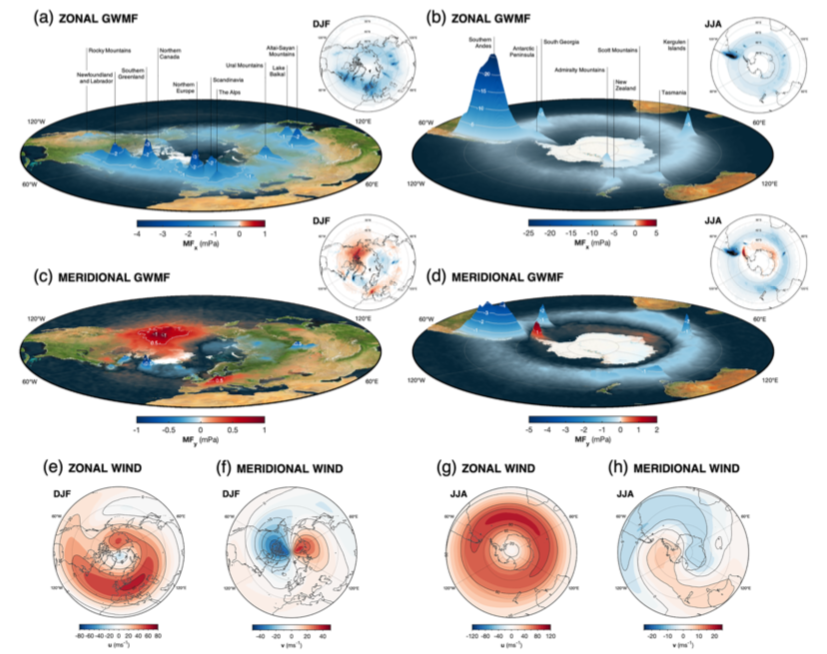
\includegraphics[width=0.85\textwidth]{figures_intro/hindley_2020_GWMF.png}
    \caption{Stereographic maps of average wintertime zonal (a, b) and meridional (c, d) GWMF near \SI{40}{\kilo\meter} altitude derived from AIRS/Aqua 3D satellite observations for the period 2002-2019. Winter is defined from December to February (June to August) for the Northern (Southern) Hemisphere. Gravity wave momentum flux values that are close to zero have been made transparent to reveal the surface features below, and landmarks that lie beneath regions of increased GWMF have been labeled. Inset in the top right of each panel is a stereographic map of the same data but centered on the north and south poles. These inset panels share a color scale with the corresponding 3D contours. Panels (e)-(h) show average wintertime zonal and meridional winds at 3 hPa for the period 2002-2019 from ERA5 reanalysis. Figure is taken from \cite{hindley_18year_2020}.}
    % Panels (e)–(h) show average wintertime zonal and meridional winds at 3 hPa for the period 2002–2019 from ERA5 reanalysis.
    \label{fig:hindley_2020_GWMF}
    %% change figure to southern hemisphere and include observational filter, then state ern 2018 observational filter better for shorter vertical wavelengths still observe GW belt (hindley discusses this in 2019 paper!!!!
    %Stratospheric zonal and meridional GWMF are illustrated on top of a map of the southern hemisphere. GWMF is derived from Atmospheric Infrared Sounder (AIRS) measurements between 2002 and 2019. Illustrated is the average over the austral winter months June – August. The figure is taken from Hindley et al. (2020))
\end{figure*}
%
The increasing number of GW observations from satellites (\cite{hindley_gravity_2019}, \citeyear{hindley_18year_2020}), ground-based lidar systems (\cite{kaifler_lidar_2020} and  \cite{kaifler_compact_2021}), aircraft (\cite{rapp_southtrac-gw_2021} and \cite{fritts_deep_2016}) and  balloons (\cite{plougonven_gravity_2013}) help to constrain GW parameterisations, but also reveal their deficiencies and point out gaps in our current theoretical knowledge on GWs. A phenomenon that was already visible in observations by \textcite{wu_satellite_1996}, but still lacks a conclusive explanation, is a GW belt around $60 \degree$S during the austral winter. It is illustrated in parts (b) and (d) of Figure \ref{fig:hindley_2020_GWMF} from \textcite{hindley_18year_2020}, who provide an extensive overview on seasonally averaged multi-year gravity wave momentum flux (GWMF) derived from satellite observations. \\
Orography undoubtedly leads to the GW hot spot between $55 \degree$W and $80 \degree$W above the southern Andes and the Antarctic Peninsula, but it only contributes about $25 \%$ to the total GWMF within the latitude band from $35 \degree$S to $68 \degree$S as stated by \textcite{hindley_18year_2020}. Following \textcite{sato_gravity_2012} and accounting for a far downstream propagation of GWs excited by the Andes, the observable GWMF in the East of the defined longitude region could be allocated to this predominantly local source, too. However, this does not heavily affect the argument of \textcite{hindley_18year_2020} that about $75 \%$ of zonal and meridional GWMF are observed at remaining longitudes over the Southern Ocean mostly peaking around $60 \degree$S (\cite{hindley_18year_2020}). \\
It has been shown that small, mountainous islands contribute to this oceanic GWMF (\cite{garfinkel_effect_2018}; \cite{mclandress_is_2012}, \cite{alexander_momentum_2009}), but again they only result in local peaks as indicated in Fig. \ref{fig:hindley_2020_GWMF}b. So non-orographic origins of GWs are most likely the reason for the wide-spread, belt-like structure of the GWMF (\cite{hendricks_what_2014}). Jet streams and fronts most likely contribute to the observed momentum flux (\cite{plougonven_internal_2014} and \cite{hendricks_what_2014}) and have also been investigated on the basis of idealized simulations (\cite{osullivan_generation_1995}). \textcite{polichtchouk_sensitivity_2018} analysed the sensitivity of high-resolution atmospheric models to non-orographic GW parameterisations and concluded a significant dependence in the same manner as \textcite{choi_effects_2013} showed that convective gravity wave drag parameterisations (a specific non-orographic source) can have a significant influence on global climate models. In addition, \textcite{jewtoukoff_comparison_2015} were able to assign wave signatures in their balloon observations to non-orographic sources, but so far none of the discussed mechanisms provides a comprehensive explanation of the wide spread observation of GWs over the Southern Ocean in the austral winter and it is still possible that some important mechanisms have not yet been considered.

The gravity wave belt around 60$\degree$S gained crucial relevance since \textcite{mclandress_is_2012} suggested its connection to the longstanding cold pole problem found in nearly all modern GCMs and chemistry climate models (CCMs). During the southern hemisphere winter months a polar vortex or polar night jet (PNJ) develops around 60$\degree$S high up in the stratosphere characterized by strong zonal westerly winds. GCMs and CCMs overestimate this PNJ, which also entails lower stratospheric temperatures over the pole compared to observations (\cite{butchart_multimodel_2011}, \cite{geller_comparison_2013} and \cite{eyring_sparc_2010}). As a result, the polar vortex breaks down too late in the spring with significant consequences on, for example, the simulated ozone trends in the Antarctic middle stratosphere (\cite{stolarski_ozone_2006}). The Antarctic ozone hole persists too long into the late spring and since Antarctic ozone depletion is the primary driver of recent southern hemisphere summertime climate change (e.g. \cite{arblaster_contributions_2006}), a delay in the vortex breakdown impacts the timing of the simulated tropospheric response. \\
\textcite{mclandress_is_2012} showed through their simulations that missing gravity wave drag from parameterisations can explain this substantial zonal wind bias around 60°S and the directly related "cold pole". A deeper understanding of the key processes that lead to the observed gravity wave belt during the austral winter could significantly improve GW parameterisations and ultimately improve long-term climate predictions through more realistic and robust GCMs. 

% include polar vortex image to show zonal wind distribution.

% or if it ultimately is a superposition of all known sources.

% temperature measurements of satellite
% in the vicinity of the 60°S belt

\section{The excitation of GWs above tropopause depressions}
\label{sec:excitation}
As outlined in the previous section, non-orographic GW sources have already been investigated from various perspectives, but are not yet able to fully explain the consistent, wide-spread appearance of GWs around 60$\degree$S. Based on observations and the analysis of high-resolution ERA5 data, \textcite{dornbrack_stratospheric_2022} propose a new mechanism that has the potential to fill this gap. They suggest an excitation of GWs above propagating tropopause depressions (TDs) in the stratosphere similar to the excitation of GWs above surface obstacles in the troposphere.

Though various definitions of the tropopause exist, all rely on abrupt changes in physical or chemical properties when transitioning from a weakly stratified troposphere ($N^2 \approx \SI{1e-4}{s^{-2}}$) to a strongly stratified stratosphere ($N^2 \approx \SI{4e-4}{s^{-2}}$) (\cite{birner_fine-scale_2006}). Common definitions are based on the thermal stratification (negative temperature lapse rate in the troposphere, positive  lapse rate in the stratosphere; \cite{wmo_meteorology_1957}), refer to the dynamical tropopause using Ertel's potential vorticity (\cite{wmo_atmospheric_1986}) or rely on chemical tracers like ozone. Despite fundamental differences in those approaches, each supports the simplification of treating the tropopause as an impermeable boundary, which is definitely not true, but a good approximation for idealized investigations. 

In the vicinity of jet streams or upper level frontal zones and associated with baroclinic processes the extratropical tropopause experiences deflections or even undergoes a folding process as visualized in Fig. \ref{fig:skerlakFold}. Dry stratospheric air penetrates down into the troposphere and folds underneath the warm air towards the equator (here northward for southern hemisphere) for deep depressions. % Potentially warmer stratospheric air
%
\begin{figure*}[t]
    \centering
    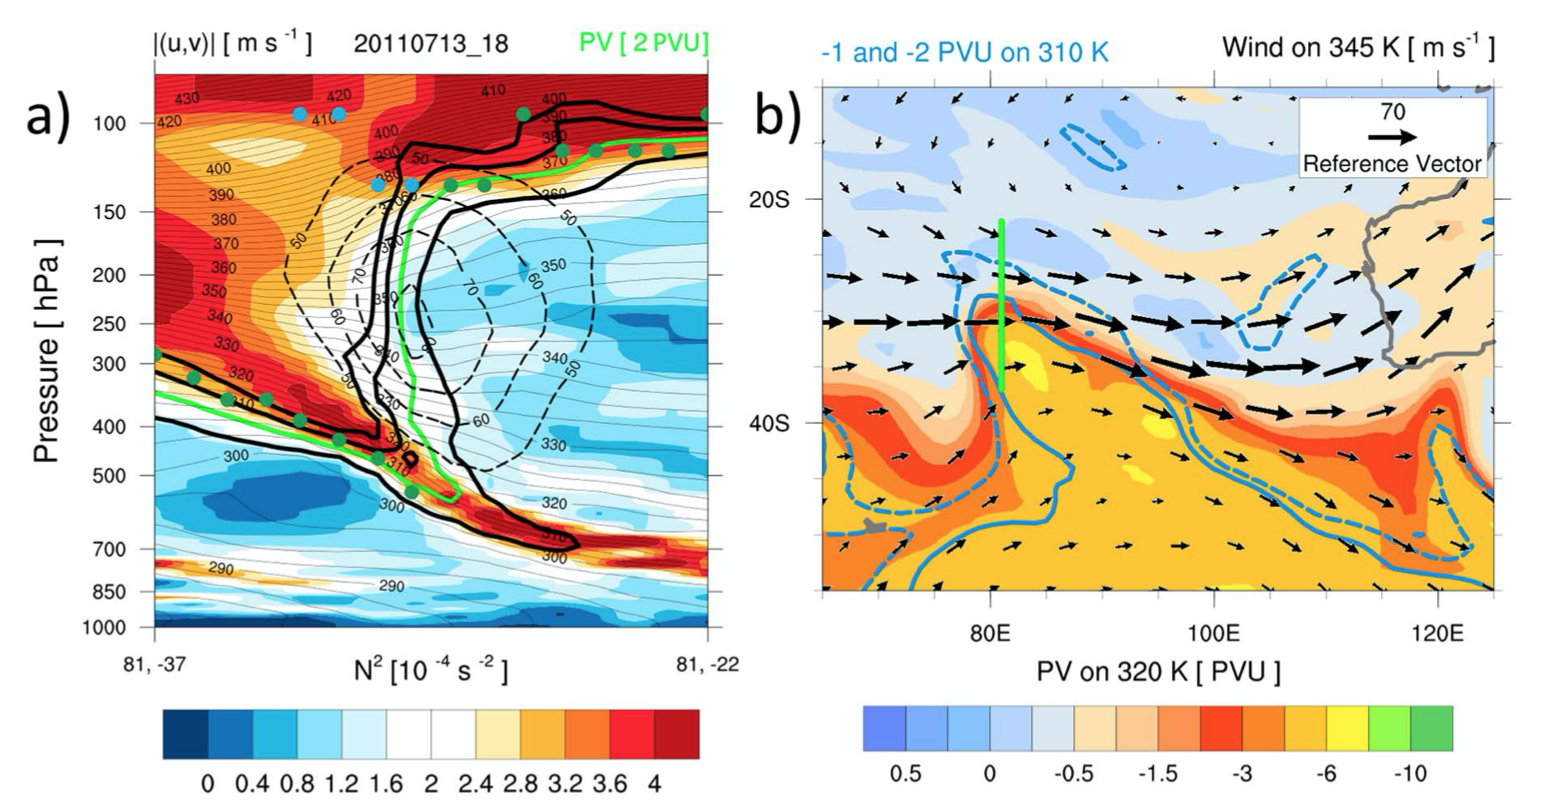
\includegraphics[width=0.9\textwidth]{figures_intro/Skerlak_Fold.png}
    \caption{Example of a deep tropopause fold near the subtropical jet west of Australia at 18 UTC on 13 July 2011. The vertical cross section shown in Figure 2a is aligned along 81$\degree$E from 37S$\degree$ to 22$\degree$S (green line segment in Figure 2b). Displayed are (a) the squared Brunt-Vaisala frequency ($N^2$, colored), potential vorticity (-1 to -4 PVU, thick solid lines, -2 PVU in green, rest in black), the WMO first and second tropopauses (green and blue solid circles, respectively), horizontal wind speed (in \SI{1}{\meter\second^{-1}}, dashed contours), and isentropes (in K, thin contours) and (b) PV on 320 K (colored, in PVU), contours of PV on 310 K at -1 PVU and -2 PVU (dashed and solid blue, respectively), and horizontal wind speed on 345K (reference vector in the top right, in \SI{1}{\meter\second^{-1}}). The West Coast of Australia is visible as grey contour. Taken from \cite{skerlak_tropopause_2015}.}
    \label{fig:skerlakFold}
\end{figure*}
%
The shape of the TD and especially the vertical extend of the prominent tongue of stratospheric air can vary significantly depending on the large scale flow conditions and strength of the upper level frontal system. This has already been discussed extensively from an observational (e.g. \cite{shapiro_further_1978} and \cite{keyser_review_1986}) and model (\cite{skerlak_tropopause_2015}) perspective. \\
Fortunately, the excitation of GWs above such a depression might not be very sensitive to the fold's shape far below the tropopause. Isentropes, that are deflected downwards, but rise again on the other side of the depression (e.g. 360-\SI{390}{\kelvin} in Figure \ref{fig:skerlakFold}a) are the ones of interest for the proposed mechanism because they mimic the flow over orography, or more precisely a valley. In addition, the zonal shape of the depression is more important for the GW forcing. This along-stream cross section (orthogonal on Figure \ref{fig:skerlakFold}a) is rarely discussed in the literature, because the main folding process happens in the cross-stream direction. Consequently, an estimate of realistic dimensions is based on the ERA5 case study by \textcite{dornbrack_stratospheric_2022} and further ERA5 analyses of cases discussed in Chapter \ref{cha:lidar} (e.g. Figure \ref{fig:era5_2018}). \textcite{dornbrack_stratospheric_2022} indicates the zonal shape of the investigated tropopause fold during their measurement campaign in the lower plots of Figure \ref{fig:RF25_era5_vertical}. The zonal width at half maximum of the propagating TD, and specifically of continuous isentropes above the tropopause, are estimated between $4 \degree$ and $12 \degree$, which transfers to a width of $240-$\SI{720}{\kilo\meter} ($1\degree \approx$ \SI{63}{\kilo\meter} at $55 \degree$S). \\
In an idealized scenario with constant background wind $U$ and Brunt–Väisälä frequency $N$ such "mountain widths" would be expected to excite waves within the hydrostatic and rotating wave regime. The advection time for an air parcel to pass over the mountain $\tau_a = \frac{a}{U}$ is comparable in magnitude to the period of inertial oscillation due to Earth’s rotation ($\tau_f = \frac{2 \pi}{f}$) with the Coriolis parameter $f \approx 10^{-4}$\SI{}{\second^{-1}} for mid-latitudes. So the Rossby number
% Thus, the time it takes for a fluid particle to cross the ridge is much larger than the period of a buoyancy oscillation
% We notice that τf /τa = 2πU/(fa) ≈ Ro
\begin{equation}
    Ro = \frac{U}{f a} \approx \frac{\tau_f}{\tau_a} \approx 2 \pi
\end{equation}
%
is close to $O(1)$ and Coriolis forces can no longer be neglected. Together with the buoyancy forces they act together as restoring forces resulting in both horizontal and vertical oscillations, which are called hydrostatic inertia-gravity waves (IGWs) (e.g. \cite{gill_atmosphere-ocean_1982} and \cite{lin_mesoscale_2007}).
% Froude number for linear non-linearity with height!!
% $L N U^{-1}$
% should be 60 m/s wind or 100km wide depression for hydrostatic scenario

A major difference of NOGWs above TDs to classic mountain waves is the transient nature of their source. \textcite{pfister_gravity_1993} already investigated the propagation of waves in the stratosphere due to a transient forcing by exposing the background flow to a time-varying obstacle, but only lifted and receded the bottom of the stratosphere. Here, a tropopause fold travels eastward with the phase speed of the Rossby wave, so the relative motion of the stratospheric air aloft to the depression's propagation speed is responsible for the excitation of the GWs. In other words, the propagating TD acts like an obstacle to the seasonally much faster stratospheric flow above. Consequently, the strong zonal winds in the stratosphere due to the PNJ during austral winter can be interpreted as a prerequisite for the excitation of NOGWs above tropopause depressions. During austral summer winds in the stratosphere are too weak and the excitation of such GWs is suppressed. \\
Simulations conducted by \textcite[]{prusa_propagation_1996} and \textcite[]{prusa_all-scale_2003} with a transient and horizontally moving lower boundary that mimics the tropopause went into that direction, but they focused on different aspects in a 2D plane. We follow a similar approach and focus on simulations of the stratosphere with the tropopause as a frictionless, impermeable lower boundary and stick to full 3D simulations to correctly represent IGWs with vertical and meridional oscillations. 

\section{The propagation of GWs above tropopause depressions}
\label{sec:propagation}
Considering the hydrostatic nature of GWs excited by TDs, the strongest wave signal should more or less appear directly above a propagating depression. And in fact, \textcite{dornbrack_stratospheric_2022} observed exactly this feature in ERA5 data, when analysing lidar measurements from the DEEPWAVE research flight 25. In Figure \ref{fig:RF25_era5_vertical}, clear wave signals mimic the appearance of mountain waves (MWs) by leaning into the westerly wind and steepening in the positive shear of the PNJ. They are observed directly above the tropopause fold for the timestamps visualized and for the whole time series between them. This builds up confidence in the proposed mechanism of a "moving valley" and suggests that GWs can be observed along the whole path of a baroclinic system responsible for a TD. \\
%
\begin{figure*}[t]
    \centering
    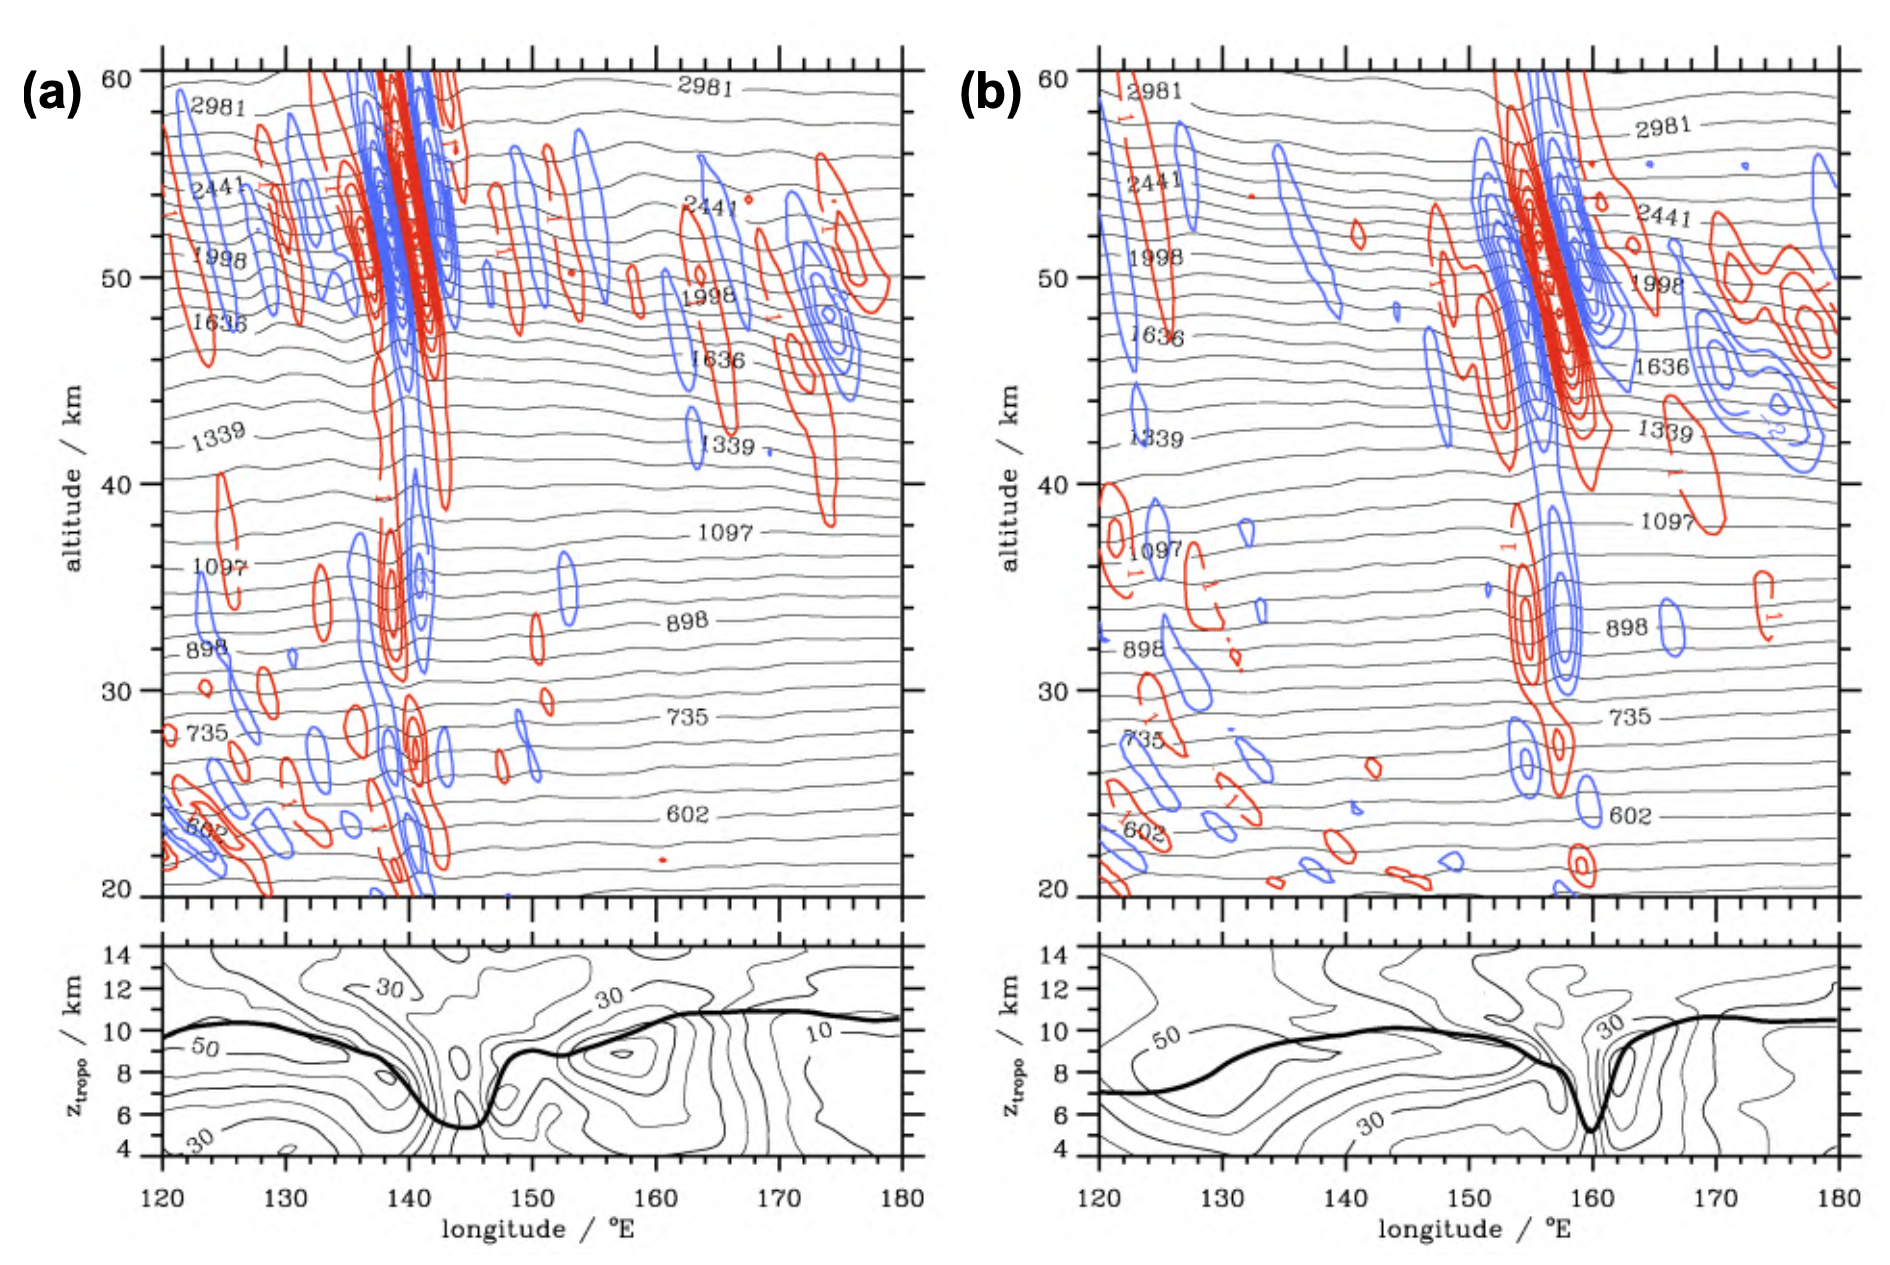
\includegraphics[width=0.99\textwidth]{figures_intro/RF25_ERA5_vertical.png}
    \caption{Temperature perturbations (K, red and blue contour lines) and potential temperature (K, black lines in logarithmic scaling) along 55$\degree$S on 17 July 2014 15 UTC (a) and 18 July 2014 09 UTC (b). The bottom panels depict the height of the dynamical tropopause (thick black lines, meridional average from 52.5$\degree$S to 57.5$\degree$S) and the horizontal wind (\SI{}{\meter\second^{-1}}, thin black lines) at the same instances. Data: One hourly ERA5 data. Taken from \textcite[]{dornbrack_stratospheric_2022}.}
    \label{fig:RF25_era5_vertical}
\end{figure*}
\begin{figure*}[t]
    \centering
    \includegraphics[width=0.99\textwidth]{figures_intro/RF25_ERA5_horizontal.png}
    \caption{Temperature perturbations $T'$ (K, color shaded) and geopotential height z (m, burgundy solid lines) at (a) 1, (b) 5, (c) 10, and (d) \SI{30}{hPa} at \SI{0900}{UTC} 18 Jul 2014. Data: ERA5 on a 0.28125° regular latitude-longitude grid. Taken from \textcite[]{dornbrack_stratospheric_2022}.}
    \label{fig:RF25_era5_horizonal}
\end{figure*} 
At this point, we note that pronounced baroclinic or frontal systems with tropopause folds in the southern hemisphere are not deviating significantly from a latitude band between 30-55$\degree$S (\cite{skerlak_tropopause_2015}). So how can NOGWs above these propagating tropopause folds explain the wave belt above the Southern Ocean centered further south at approximately 60°S in Figure \ref{fig:hindley_2020_GWMF}b and \ref{fig:hindley_2020_GWMF}d? The last piece to the puzzle is the meridional propagation of GWs in the stratosphere. \\
Two mechanisms can cause such a meridional propagation. At first, the orientation of the TDs is rarely north-south resulting in a slightly inclined wave vector with respect to the predominantly westerly flow in the upper stratosphere. The wave vector ($k$,$l$) defines the wave's intrinsic propagation direction and leads to a lateral deflection as soon as tilted obstacles with respect to the background flow are in place. \textcite{preusse_space-based_2002} for example considers this mechanism for GWs excited by the Andes at similar latitudes. The second process is based on ray-tracing theory and was first discussed and applied by \textcite{dunkerton_inertiagravity_1984}. It describes the modification of the meridional wavenumber by the background wind with
\begin{equation}
    \frac{dl}{dt} = -(k \frac{\partial U}{\partial y} + l \frac{\partial V}{\partial y} + \frac{\beta f}{\hat{\omega}})
    \approx -k \frac{\partial U}{\partial y}.
    \label{equ:meridionalRefraction}
\end{equation}
In a simplified scenario with purely zonal background flow ($V=0$) and no gradient of the Coriolis force $f$ ($\beta=0$), $\frac{dl}{dt}$ along the ray is proportional to the meridional gradient of the background wind $U$ and the zonal wavenumber $k$. In other words, meridional wind shear develops a meridional component of the wave vector even in the case of a purely zonal initial propagation. In general, this phenomenon leads to a refraction of internal GWs into the southern hemispheric PNJ at 60$\degree$S illustrated in Figure \ref{fig:hindley_2020_GWMF}g. It has already been described by a number of publications (e.g. \cite{dunkerton_inertiagravity_1984}, \cite{preusse_space-based_2002}, \cite{sato_origins_2009}, \cite*{sato_gravity_2012}, \cite{ehard_horizontal_2017} and \cite{jiang_stratospheric_2019}). \textcite{jiang_stratospheric_2019} further add, that waves are elongated towards the stronger background wind (towards the center of the PNJ) and shortened on the opposite side with weaker winds. \\
A zonally elongated GW pattern in the upper stratosphere is also present during the event in Figure \ref{fig:RF25_era5_vertical} by \textcite[]{dornbrack_stratospheric_2022}. Figure \ref{fig:RF25_era5_horizonal} shows corresponding horizontal cross sections at different pressure levels and at all heights phase lines have a very significant meridional wave vector component $l$. It seems that GWs are excited over the Southern Ocean somewhere southwest of Australia, then propagate up and south into the PNJ while getting refracted by the jet's shear. Especially at 1 and \SI{5}{hPa} in (a) and (b) the zonal extend of the elongated phase line pattern is very large, so one goal of this thesis will be a demonstration that NOGWs above tropopause folds can cause such a GW pattern within the southern hemisphere winter stratosphere.  

\section{Research goals and outline}
\label{sec:goals}
It is the overarching goal of this Master's thesis to take up the hypothesis of \textcite[]{dornbrack_stratospheric_2022} and demonstrate that their proposed excitation mechanism of GWs above tropopause depressions can indeed explain individual observations of GWs in the upper stratosphere and contribute to the GW belt in the southern hemisphere winter stratosphere. Various different properties of the tropopause and the stratospheric environment will have a significant positive or negative influence on the excitation and propagation of these NOGWs, so a comprehensive sensitivity study based on idealized numerical simulations provides the basis for this investigation. In these simulations an impermeable, frictionless, transient lower boundary mimics the tropopause to simplify the simulation and focus on properties of the tropopause and on properties of the stratospheric environment. In a first step, we simplify even more and conduct computationally less expensive simulations with a coarse resolution in meridional direction and focus on zonal and vertical characteristics to answer our first research question in Chapter \ref{sec:resultsQ3D}.
\begin{tcolorbox}[]
    (R1) How sensitive are NOGWs from propagating tropopause depressions to the depression's 2D shape and to properties of the stratospheric environment?
\end{tcolorbox}
Naturally, more complex simulations with an identical resolution in zonal and meridional direction follow in Chapter \ref{sec:results3D} and we focus on meridional aspects of the tropopause and the meridional propagation of GWs within the stratosphere to answer the second research question of this thesis.
\begin{tcolorbox}[]
    (R2) How sensitive are NOGWs from propagating tropopause depressions to the depression's 3D shape and meridional variations of the stratospheric airflow?
\end{tcolorbox}
The simulations in Chapter \ref{sec:results3D} also facilitate the investigation of the third research question, which refers to the zonally elongated phase lines in the horizontal cross sections of Figure \ref{fig:RF25_era5_horizonal}. As anticipated in the previous section, it is one goal of this thesis to check if the proposed excitation mechanism can also replicate the zonally elongated GW pattern (Figure \ref{fig:RF25_era5_horizonal}) in the stratosphere above the Southern Ocean described in the case study by \textcite[]{dornbrack_stratospheric_2022}. The third research question is also addressed in Chapter \ref{sec:results3D}. % and implies the identification of necessary properties to ob. 
\begin{tcolorbox}[]
    (R3) Can NOGWs above propagating tropopause depressions explain the zonally elongated phase lines in ERA5 above the Southern Ocean?
\end{tcolorbox}
% The fourth research question addresses

Multiple discussions in Chapter \ref{sec:resultsQ3D} and \ref{sec:results3D} are based on the vertical flux of horizontal momentum MF, because it is very meaningful in the context of wave-mean flow interactions in the middle atmosphere and for constraining GW parameterizations in climate simulations (e.g. \cite[]{geller_comparison_2013} or \cite[]{kim_overview_2003}). In numerical simulations MF can be calculated directly from available wind perturbations ($u'$,$v'$ and $w'$), but most satellite or ground-based instruments that provide observations of the upper atmosphere on a reasonable scale to study GWs are only capable of measuring temperature. Under certain assumptions, the MF can also be calculated from temperature perturbations and the corresponding wave's horizontal and vertical scale. Chapter \ref{sec:mf_comp} provides further details on these assumptions and investigates whether GWs above tropopause depressions fulfill them by answering research question 4:
\begin{tcolorbox}[]
    (R4) Can the MF of NOGWs above propagating tropopause depressions be calculated from temperature perturbations?
\end{tcolorbox}

The last research question links the idealized simulations of this thesis to available GW observations in the stratosphere, in particular, to ground-based lidar observations. Regular observations of GWs in this region are sparse, and for now, only a small number of ground-based lidar stations and satellite instruments (e.g AIRS onboard NASA's Aqua satellite) are currently operational and provide limited observations (e.g. \cite[]{kaifler_compact_2021} and \cite[]{hindley_18year_2020}). Ground-based lidar stations obtain vertical timeseries with a high temporal and vertical resolution. These can also be emulated in the idealized numerical simulations to identify characteristics of GWs above propagating TDs that might allow a differentiation to other GWs like MWs. Research question five is addressed in Chapter \ref{cha:lidar}.
\begin{tcolorbox}[]
    (R5) Can NOGWs from propagating tropopause depressions be identified in ground-based lidar observations?
\end{tcolorbox}
We can anticipate that the propagating source of the GWs implies a distinct pattern in vertical timeseries which opens the door to search for the respective pattern in actual measurements. Two observations of the Compact Rayleigh Autonomous Lidar (CORAL) currently operational in Río Grande, Argentina at 53.79°S are also discussed in Chapter \ref{cha:lidar}.

A short overview on utilized tools and on the data is given in Chapter \ref{sec:methods} and the setup of all simulations is described in Chapter \ref{sec:EULAG}.

% INCLUDE OUTLOOK OF andreas paper with suggestions for further work

% Together with the regular appearance of Rossby wave trains (baroclinic systems involving TDs) at middle latitudes in the southern hemisphere, these processes could provide a conclusive explanation for the widespread and patchy stratospheric GW activity all the way around the Southern Ocean shown in Fig. \ref{fig:hindley_2020_GWMF}b and \ref{fig:hindley_2020_GWMF}d or in the case study in Figure ref{fig:RF25_era5_horizonal}. More specifically, the Master's thesis shall answer the following research questions:

%Figure \ref{fig:RF25_era5_vertical} was motivation for analogy of excitation mechanism with MWs, so this pattern is quite likely... however horizontal cross section pattern is interesting...


% Stationary synoptic patterns like blocks are rare in the southern hemisphere, because of 

% It is clear that the flow regime above a TD is much more complicated than a zonal overflow of an elongated mountain ridge, which produces the expected hydrostatic waves aloft. Three dimensional Furthermore, the fold itself travels eastward with the phase speed of the Rossby

% impermeable boundary
% shear wind rotation with height to strong zonal wind 

% The World Meteorological Organization defines the tropopause as the lowest level where the abso- lute value of the temperature lapse rate decreases to 2K/km. or less, with the average lapse rate between this level and all higher levels within 1.2 mi. (2 km.) not exceeding 2K/km. The dynamical tropopause is defined in terms of sharp changes in the potential vor- ticity (much higher in the stratosphere), which mea- sures stratification and rotation of the air masses. An abrupt increase (decrease) with height of the ozone (water vapor) mixing ratio indicates the presence of the chemical tropopause.

% thermal definition
% dynamic definition potential temperature and pressure on the dynamic tropopause (defined here as the 1.5 × 10−6 m2 K kg−1 s−1, hereafter 1.5 PVU, Ertel PV surface)
% chemical definition

% thermal fields and wind fields

% bush vertical / horizontal aspect ratio of 0.06 penetrates the troposphere

% \cite{clark_convectively_1986} above inversion layer?? 

% state that using tropopause fold and depression meaning the same

% half width is approximately 4/5 degree and 2 degree in zonal vertical cross section Dörnbrack et al

% Significant intrusions of stratospheric air occur in “ribbons” ~200 to 100 km in length, 100 to 300 km wide and about 1 to 4 km thick (EPA 2006).